\noindent \textbf{Kode og alle plotter for innleveringen finnes i \href{https://github.com/Yonatan1717/SigB}{\textcolor{blue}{https://github.com/Yonatan1717/SigB}}.}\\[1em]
% tidsdomene → frekvensdomene → filter → tidsdomene
Min besvarelse følger følgende mønster: 
\[
   \text{tidsdomenet } \rightarrow \text{ frekvensdomenet } \rightarrow \text{ filter } \rightarrow \text{ tidsdomenet}
\]


\hypertarget{oppgave1}{}
\section*{Oppgave 1}
\addcontentsline{toc}{section}{oppgave1}

Oppgaven undersøker Fourier-serierepresentasjonen av et periodisk
rektangulært pulstog og hvordan signalet påvirkes når det sendes
gjennom et førsteordens RC-lavpassfilter. Signalet har amplitude:
\[
A = 2~\mathrm{V},
\]
pulsbredde:
\[
\tau = 2~\mathrm{ms},
\]
og periodetid:
\[
T = 8~\mathrm{ms}
\]
Grunnfrekvensen blir dermed:
\[
f_0 = \frac{1}{T}
    = \frac{1}{8\cdot10^{-3}}
    = 125~\mathrm{Hz}
\]

% --------------------------------------------------
\hypertarget{a}{}
\subsection*{a)}
Pulstoget er sentrert omkring $t=0$ og kan innenfor en periode
beskrives som:
\[
x(t)=
\begin{cases}
A, & |t| \leq \frac{\tau}{2},\\
0, & \text{ellers}.
\end{cases}
\]
Den reelle Fourier-serien skrives, med samme konvensjon som brukes
i Octave-koden, som:
\[
x(t)
=
a_0
+
\sum_{n=1}^{\infty}
\left[
a_n\cos(n\omega_0t)
+
b_n\sin(n\omega_0t)
\right] \quad \Rightarrow
\]
\[
    x(t) = a_0 + \sum_{n=1}^{\infty} A_n \cos(n\omega_0 t + \phi_n)
\]
\[
    A_n = \sqrt{a_n^2 + b_n^2}, \quad \phi_n = \arctan\frac{-b_n}{a_n}
\]
Siden signalet er symmetrisk omkring $t=0$, er det et jevnt signal.
Sinuskoeffisientene blir derfor:
\[
b_n = 0
\]
DC-komponenten beregnes som:
\[
a_0
=
\frac{1}{T}
\int_{-T/2}^{T/2}x(t)\,dt
\]
Siden signalet bare er ulik null i tidsintervallet $-\tau/2 \leq t \leq \tau/2$, får vi:
\[
a_0
=
\frac{1}{T}
\int_{-\tau/2}^{\tau/2} A\,dt
=
A \cdot \frac{\tau}{T}, \quad d_c = \frac{\tau}{T} \ (\text{duty cycle})
\]
Med verdiene fra oppgaven blir dette:
\[
a_0
=
\frac{2\cdot2\cdot10^{-3}}
     {8\cdot10^{-3}}
=
0.5~\mathrm{V}
\]
Cosinuskoeffisientene beregnes som:
\[
a_{n}
=
\frac{2}{T}
\int_{-\tau/2}^{\tau/2}
A\cos(n\omega_0t)\,dt
\]
Dette gir:
\[
a_n
=
\frac{2A}{n\pi}
\sin\left(
n\pi \cdot d_c
\right)
\]
Ved å bruke den normaliserte sinc-funksjonen:
\[
\mathrm{sinc}(x)
=
\frac{\sin(\pi x)}{\pi x},
\]
kan dette skrives som:
\[
a_n
=
2\cdot a_0 \cdot
\mathrm{sinc}
\left(
n \cdot d_c
\right)
\]
Siden:
\[
\frac{\tau}{T}
=
\frac{2}{8}
=
\frac{1}{4}
\]
og $2a_0=1$, får vi:
\[
a_n
=
\mathrm{sinc}
\left(
\frac{n}{4}
\right)
\]
Grunnvinkelfrekvensen er:
\[
\omega_0
=
2\pi f_0
=
250\pi~\mathrm{rad/s}
\]
Fourier-representasjonen blir dermed:
\[
\boxed{
x(t)
=
0.5
+
\sum_{n=1}^{\infty}
\mathrm{sinc}
\left(
\frac{n}{4}
\right)
\cos(250\pi n t)
}
\]

% --------------------------------------------------
\hypertarget{b}{}
\subsection*{b)}
De seks første harmoniske Fourier-koeffisientene beregnes numerisk
i Octave. Egne hjelpefunksjoner brukes for å beregne DC-komponenten,
amplitude og fase:
\begin{verbatim}
[dc, t_sq, sq] = findA0(func, T, dp);

[amp_l, phi_l, freq_l, a_l, b_l, amp_mm, phi_mm] = ...
    findAnandBns(func, T, N, dp); 
    % amp_l innholder liste med A_n
\end{verbatim}
Resultatet blir:
\begin{center}
\begin{tabular}{c|c|c|c}
$n$ & $f$ [Hz] & $A_{n,\mathrm{in}}$ [V] & $\phi_{n,\mathrm{in}}$ [deg] \\
\hline
0 & 0   & 0.5000  & 0 \\
1 & 125 & 0.9003  & 0 \\
2 & 250 & 0.6366  & 0 \\
3 & 375 & 0.3001  & 0 \\
4 & 500 & 0       & uDef \\
5 & 625 & 0.1801  & -180 \\
6 & 750 & 0.2122  & -180
\end{tabular}
\end{center}
Den fjerde harmoniske komponenten blir null. Dette stemmer også
med uttrykket:
\[
a_n=\mathrm{sinc}\left(\frac{n}{4}\right),
\]
siden:
\[
\mathrm{sinc}(1)=0
\]
Et negativt Fourier-ledd kan alternativt beskrives med positiv
amplitude og en faseforskyvning på $180^\circ$ (eller ekvivalent $-\!180^\circ$).

% --------------------------------------------------
\hypertarget{c}{}
\subsection*{c)}
Fourier-komponentene summeres for å rekonstruere signalet i
tidsdomenet. I programmet gjøres dette ved hjelp av funksjonen
\texttt{getTimeDomainFromSpectrum()}:
\begin{verbatim}
f_l = [0, freq_l];

unfiltered_amp_l = [dc, amp_l];
unfiltered_phi_l = [0, phi_l];

[t_fourier, yin] = getTimeDomainFromSpectrum( ...
    f_l, unfiltered_amp_l, unfiltered_phi_l, 3, 1000);
\end{verbatim}
Det opprinnelige rektangulære pulstoget og Fourier-serien med
$N=6$ er vist i figuren under:
\begin{figure}[H]
    \centering
    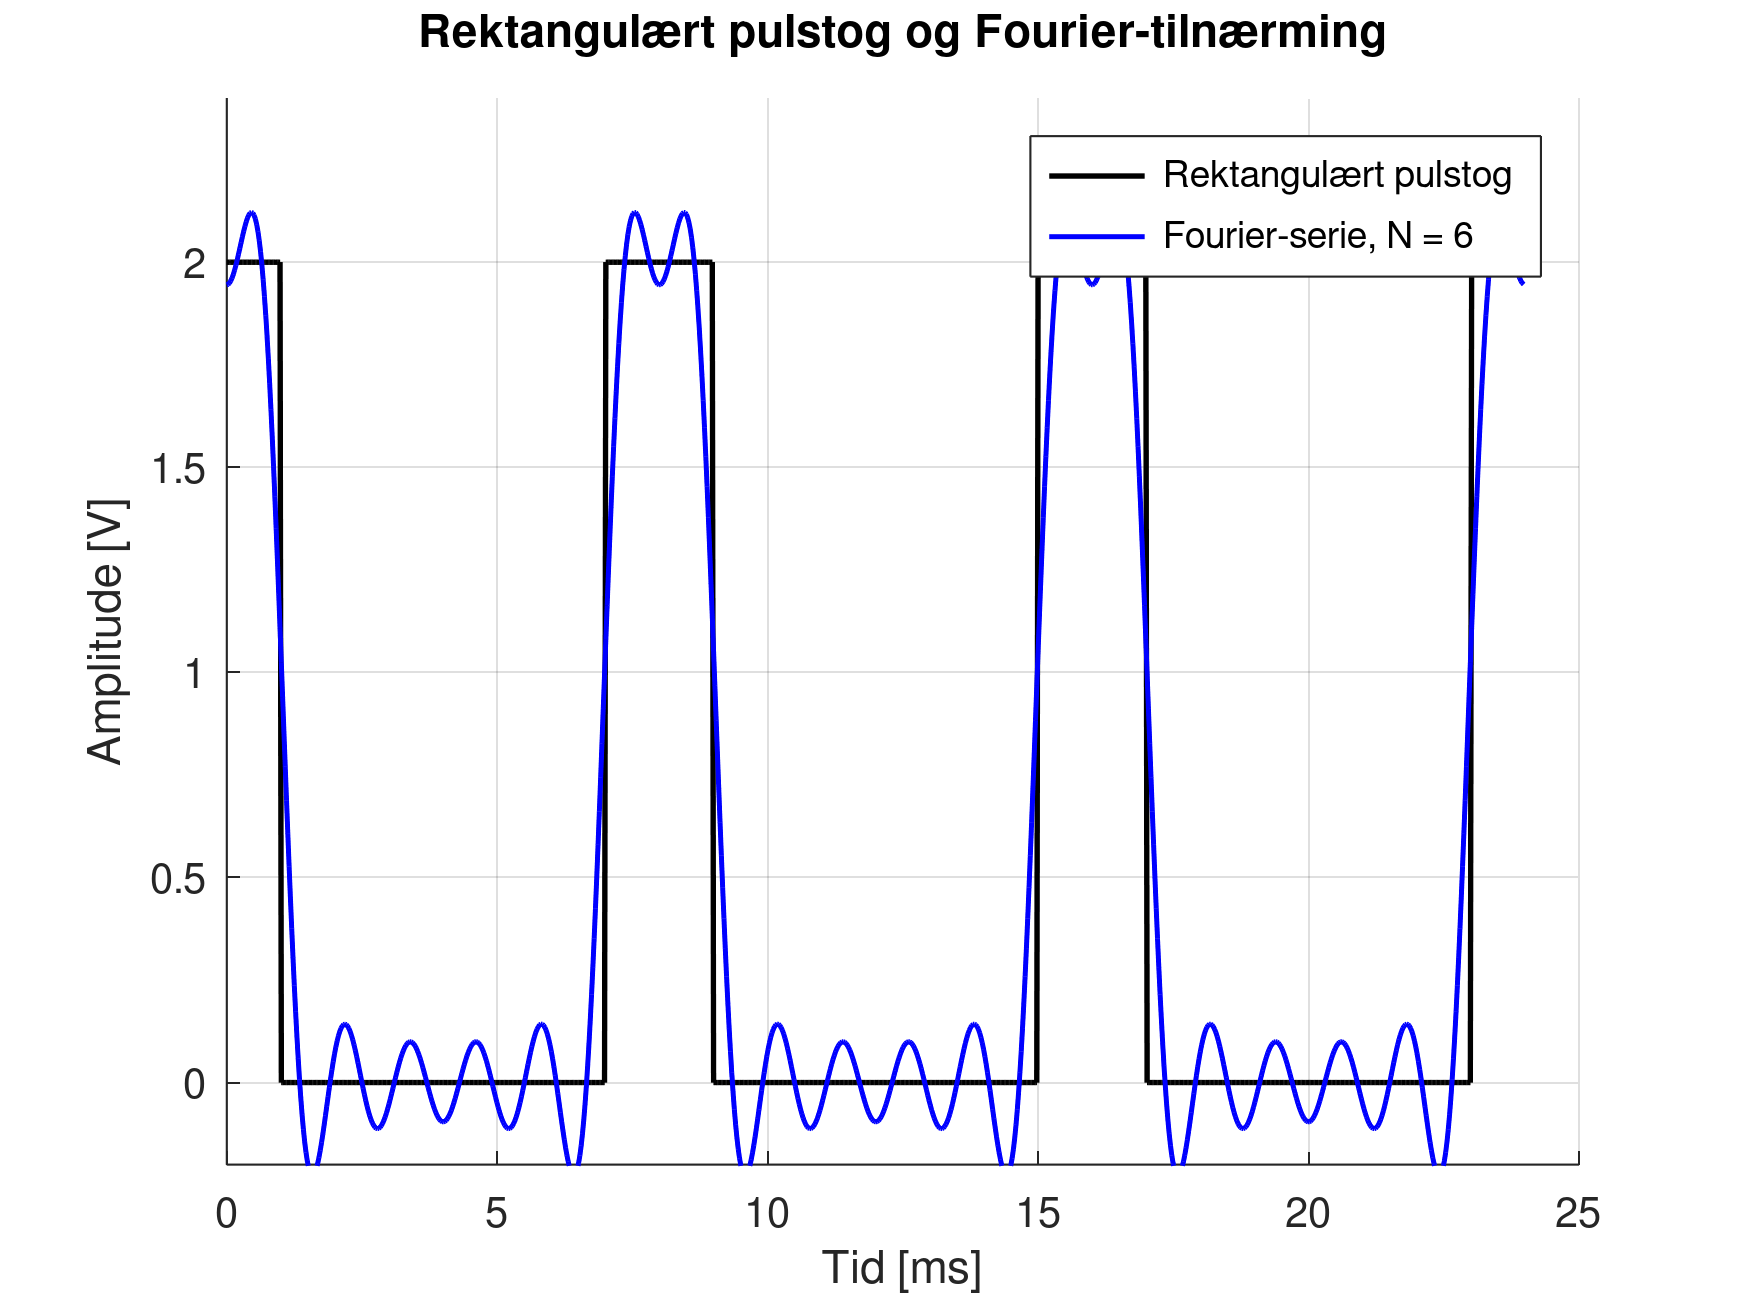
\includegraphics[width=0.85\textwidth]
    {../Media/oppgave_c_fourier_tid.png}
    \caption{Rektangulært pulstog og Fourier-serietilnærming med $N=6$.}
\end{figure}
\noindent Fourier-serien følger den generelle formen til pulstoget godt,
men det oppstår svingninger i nærheten av de brå overgangene.
Dette skyldes at signalet rekonstrueres med et begrenset antall
frekvenskomponenter. Et ideelt sprang krever i prinsippet
uendelig mange harmoniske komponenter. Amplitude- og fasespekteret for de seks første harmoniske
komponentene er vist under.
\begin{figure}[H]
    \centering
    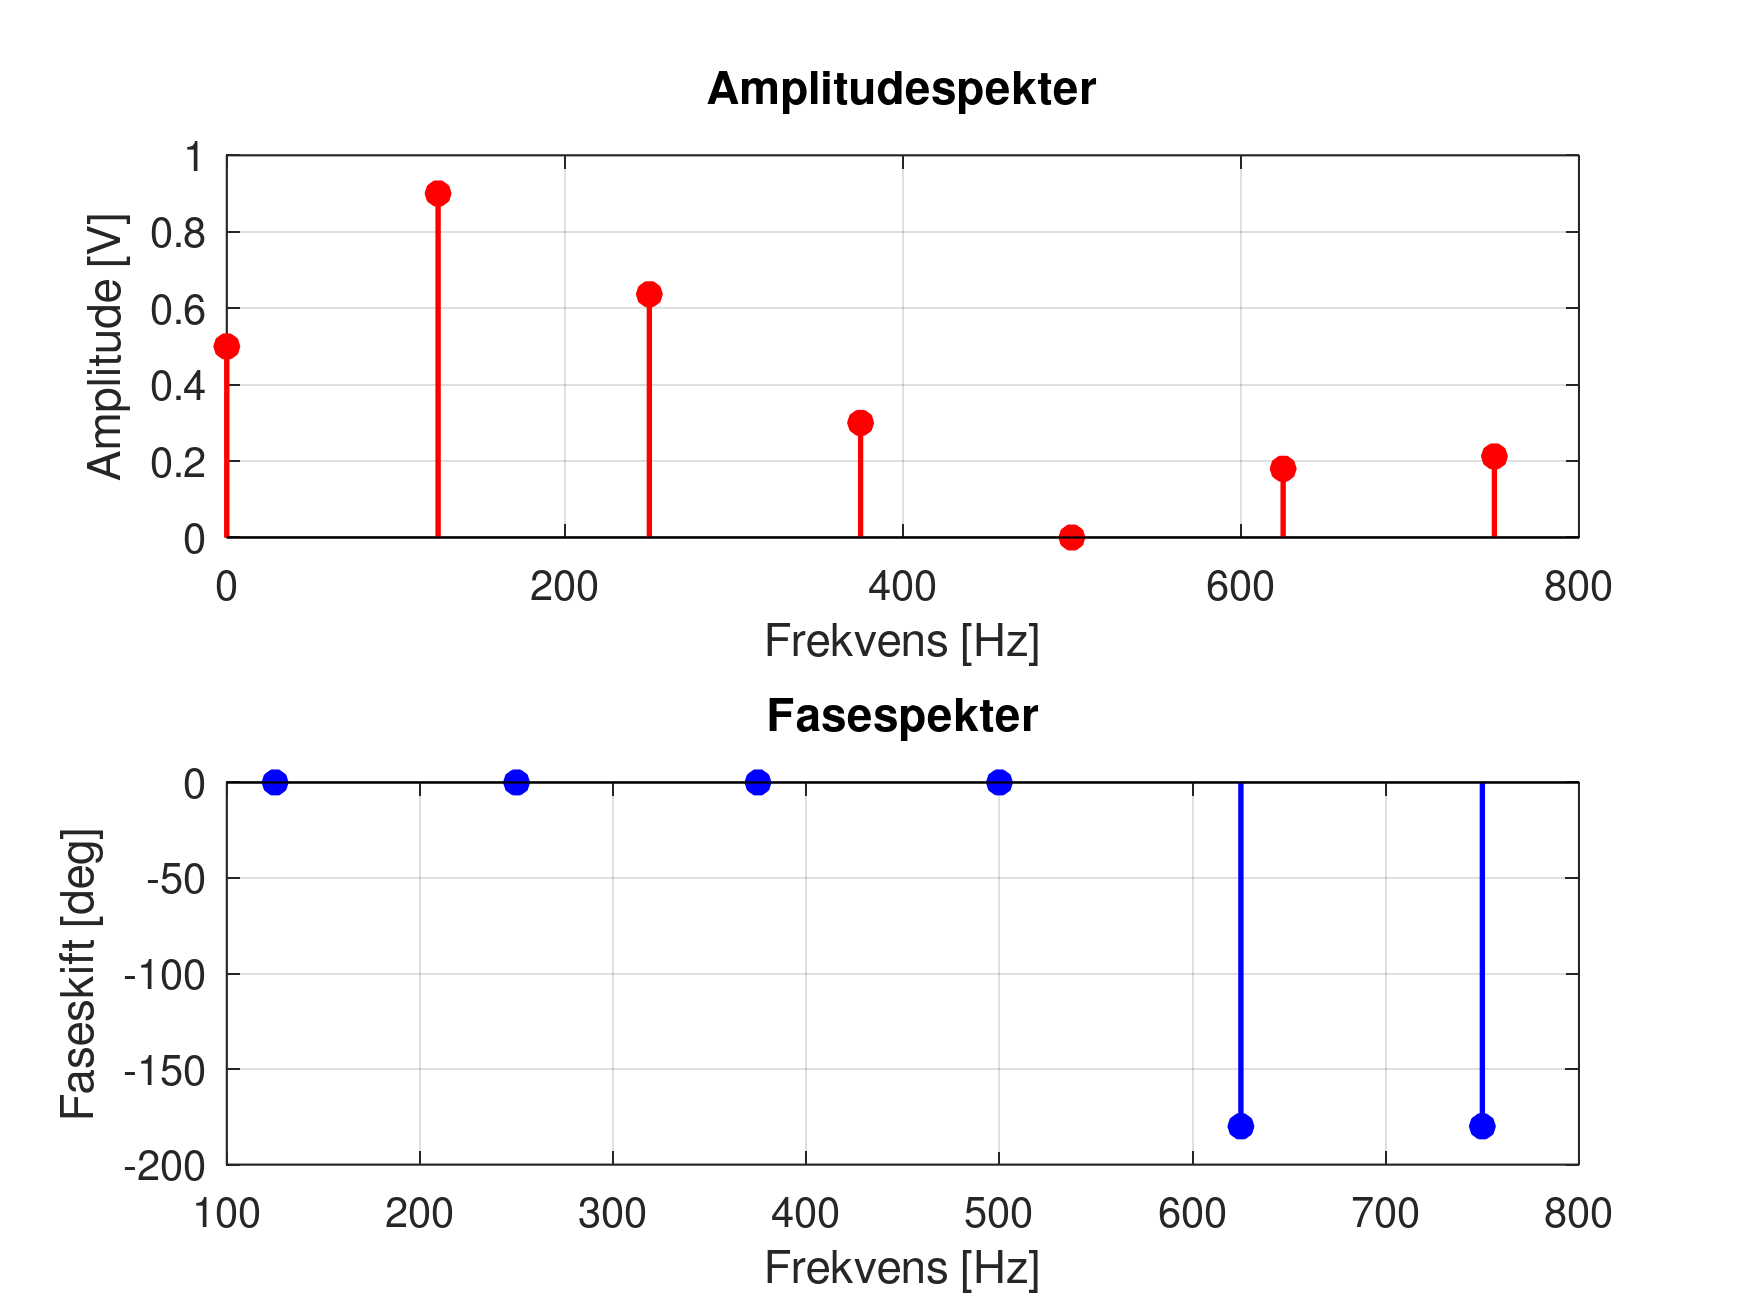
\includegraphics[width=0.85\textwidth]
    {../Media/oppgave_c_fourier_spekter.png}
    \caption{Amplitude- og fasespekter for Fourier-serien.}
\end{figure}

% --------------------------------------------------
\hypertarget{d}{}
\subsection*{d)}
Antall Fourier-komponenter har stor betydning for hvor godt
Fourier-serien representerer det opprinnelige pulstoget.\\[1em]
Når $N$ økes, tas flere av de høyfrekvente komponentene med.
Dette gir brattere slope og en bedre tilnærming til det
rektangulære pulstoget. Med få komponenter blir signalet mer
avrundet.\\[1em]
Amplituden $A$ skalerer Fourier-koeffisientene. Dersom amplituden
økes, øker både DC-komponenten og amplituden til de harmoniske
komponentene tilsvarende.\\[1em]
Pulsbredden $\tau$ bestemmer signalets duty cycle og påvirker
fordelingen av energi mellom frekvenskomponentene. En smalere
puls krever generelt flere høyfrekvente komponenter for å kunne
representeres nøyaktig, og får derfor større båndbredde. Periodetiden $T$ bestemmer grunnfrekvensen:
\[
f_0=\frac{1}{T}
\]
En større periodetid gir derfor lavere grunnfrekvens og mindre
avstand mellom de harmoniske frekvenskomponentene.

% --------------------------------------------------
\hypertarget{e}{}
\subsection*{e)}
\begin{figure}[H]
    \centering
    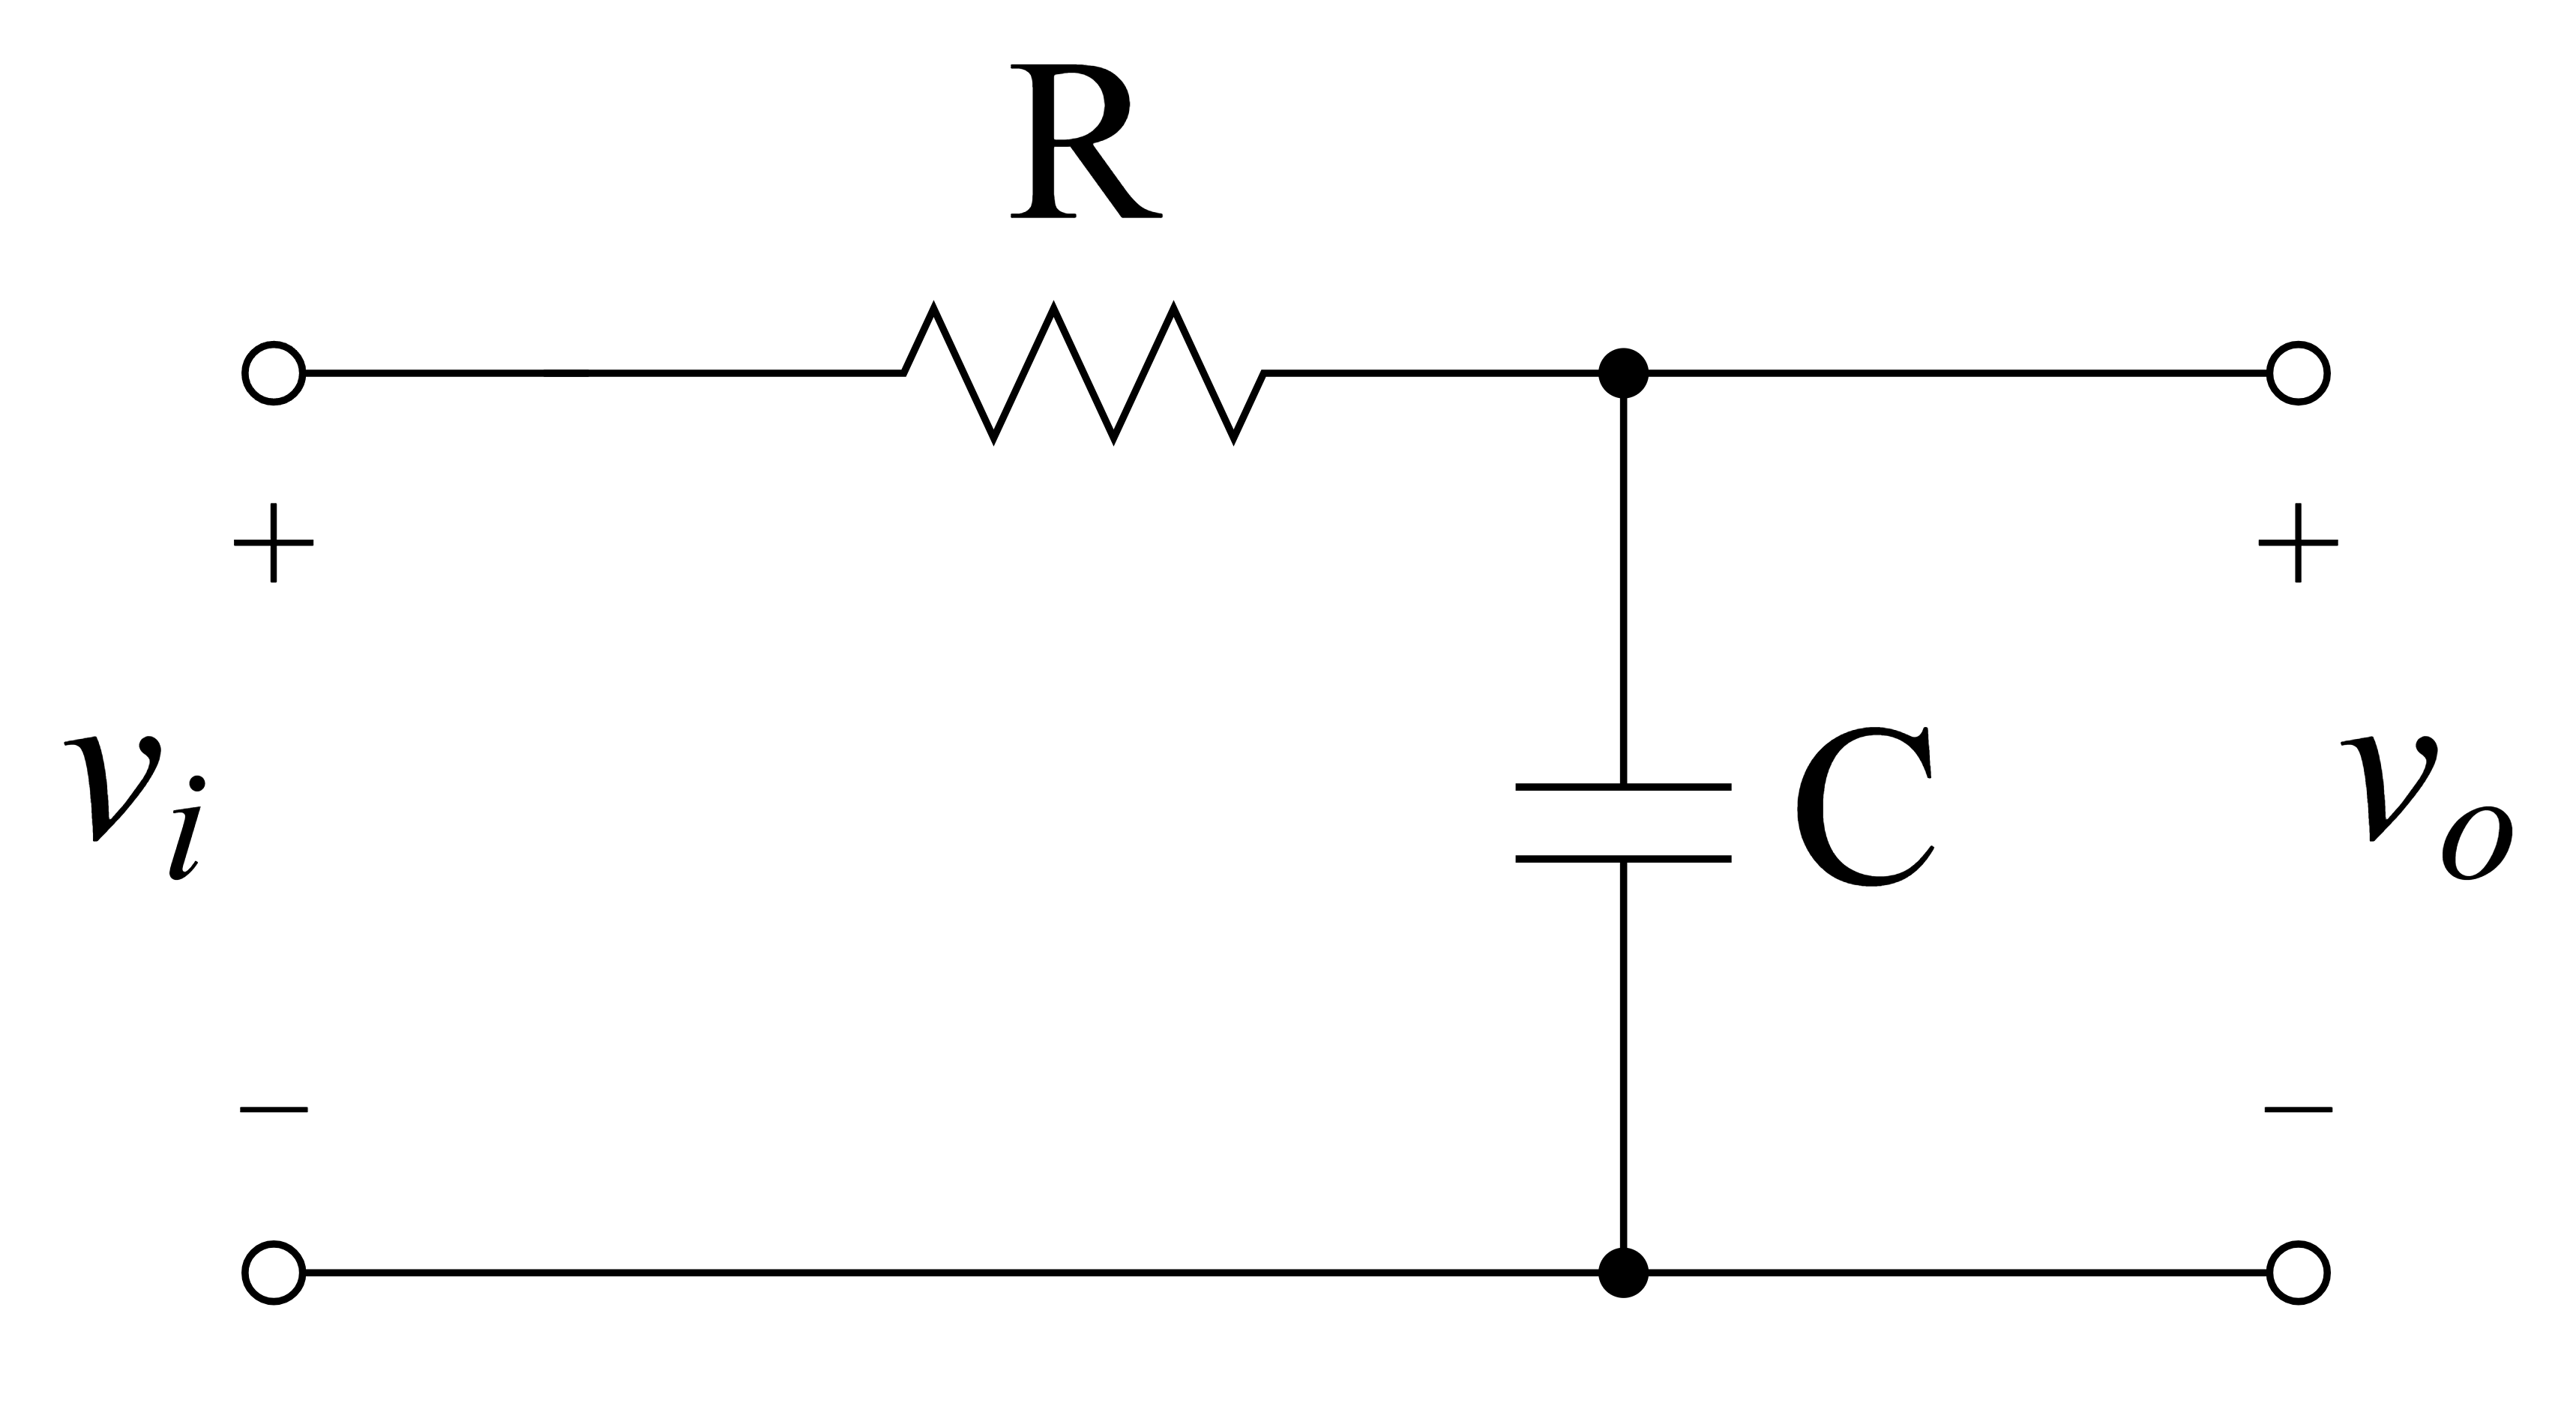
\includegraphics[width=0.75\textwidth]
    {../Media/RC.png}
    \caption{RC-lavpassfilter krets}
\end{figure}
\noindent Ved hjelp av KVL kan responsen til dette systemet beskrives med en førsteordens differensialligning:
\[
    RC\frac{dv_o(t)}{dt}+v_o(t) = v_i(t), \quad v_o(t) = v_c(t)
\]
bruker Laplace-transformasjonen og får overføringsfunksjonen:
\[
    RC \cdot (sV_o(s) - v_o(0)) + V_o(s) = V_i(s)
\]
For overføringsfunksjonen antar vi at kondensatoren er utladet ved $t=0$, dvs. $v_o(0)=0$. Dette gir:
\[
    V_o(s) \cdot (1 + sRC) = V_i(s) \quad \Rightarrow 
\]
\[
    H(s) = \frac{V_o(s)}{V_i(s)} = \frac{1}{1 + sRC}
\]
Polen til systemet ligger altså ved $s=-\frac{1}{RC}$. Ved å erstatte $s$ med $j\omega$ får vi frekvensresponsen:
\[
    H(j\omega) = \frac{1}{1+j\omega RC}
\]
Vi har da at magnituden og fasen til frekvensresponsen er gitt ved:
\[
    |H(j\omega)| = \frac{1}{\sqrt{1+(\omega RC)^2}}
\]
\[
    \angle H(j\omega) = -\arctan(\omega RC)
\]
For å finne knekkfrekvensen setter vi $|H(j\omega)| = \frac{1}{\sqrt{2}}$ og får:
\[
    \omega_c = \frac{1}{RC} \quad \Rightarrow \quad f_c = \frac{1}{2\pi RC}
\]
\clearpage
\noindent
Frekvensresponsen for de aktuelle Fourier-komponentene blir:
\begin{center}
\begin{tabular}{c|c|c}
$f$ [Hz] & $|H(f)|$ & $\angle H(f)$ [deg] \\
\hline
0   & 1.0000 & 0.00 \\
125 & 0.9701 & -14.04 \\
250 & 0.8944 & -26.57 \\
375 & 0.8000 & -36.87 \\
500 & 0.7071 & -45.00 \\
625 & 0.6247 & -51.34 \\
750 & 0.5547 & -56.31
\end{tabular}
\end{center}
Ved knekkfrekvensen $500$ Hz er amplitudefaktoren:
\[
|H(f_c)|
=
\frac{1}{\sqrt{2}}
\approx
0.707,
\]
og faseforskyvningen er $-45^\circ$.
\begin{figure}[H]
    \centering
    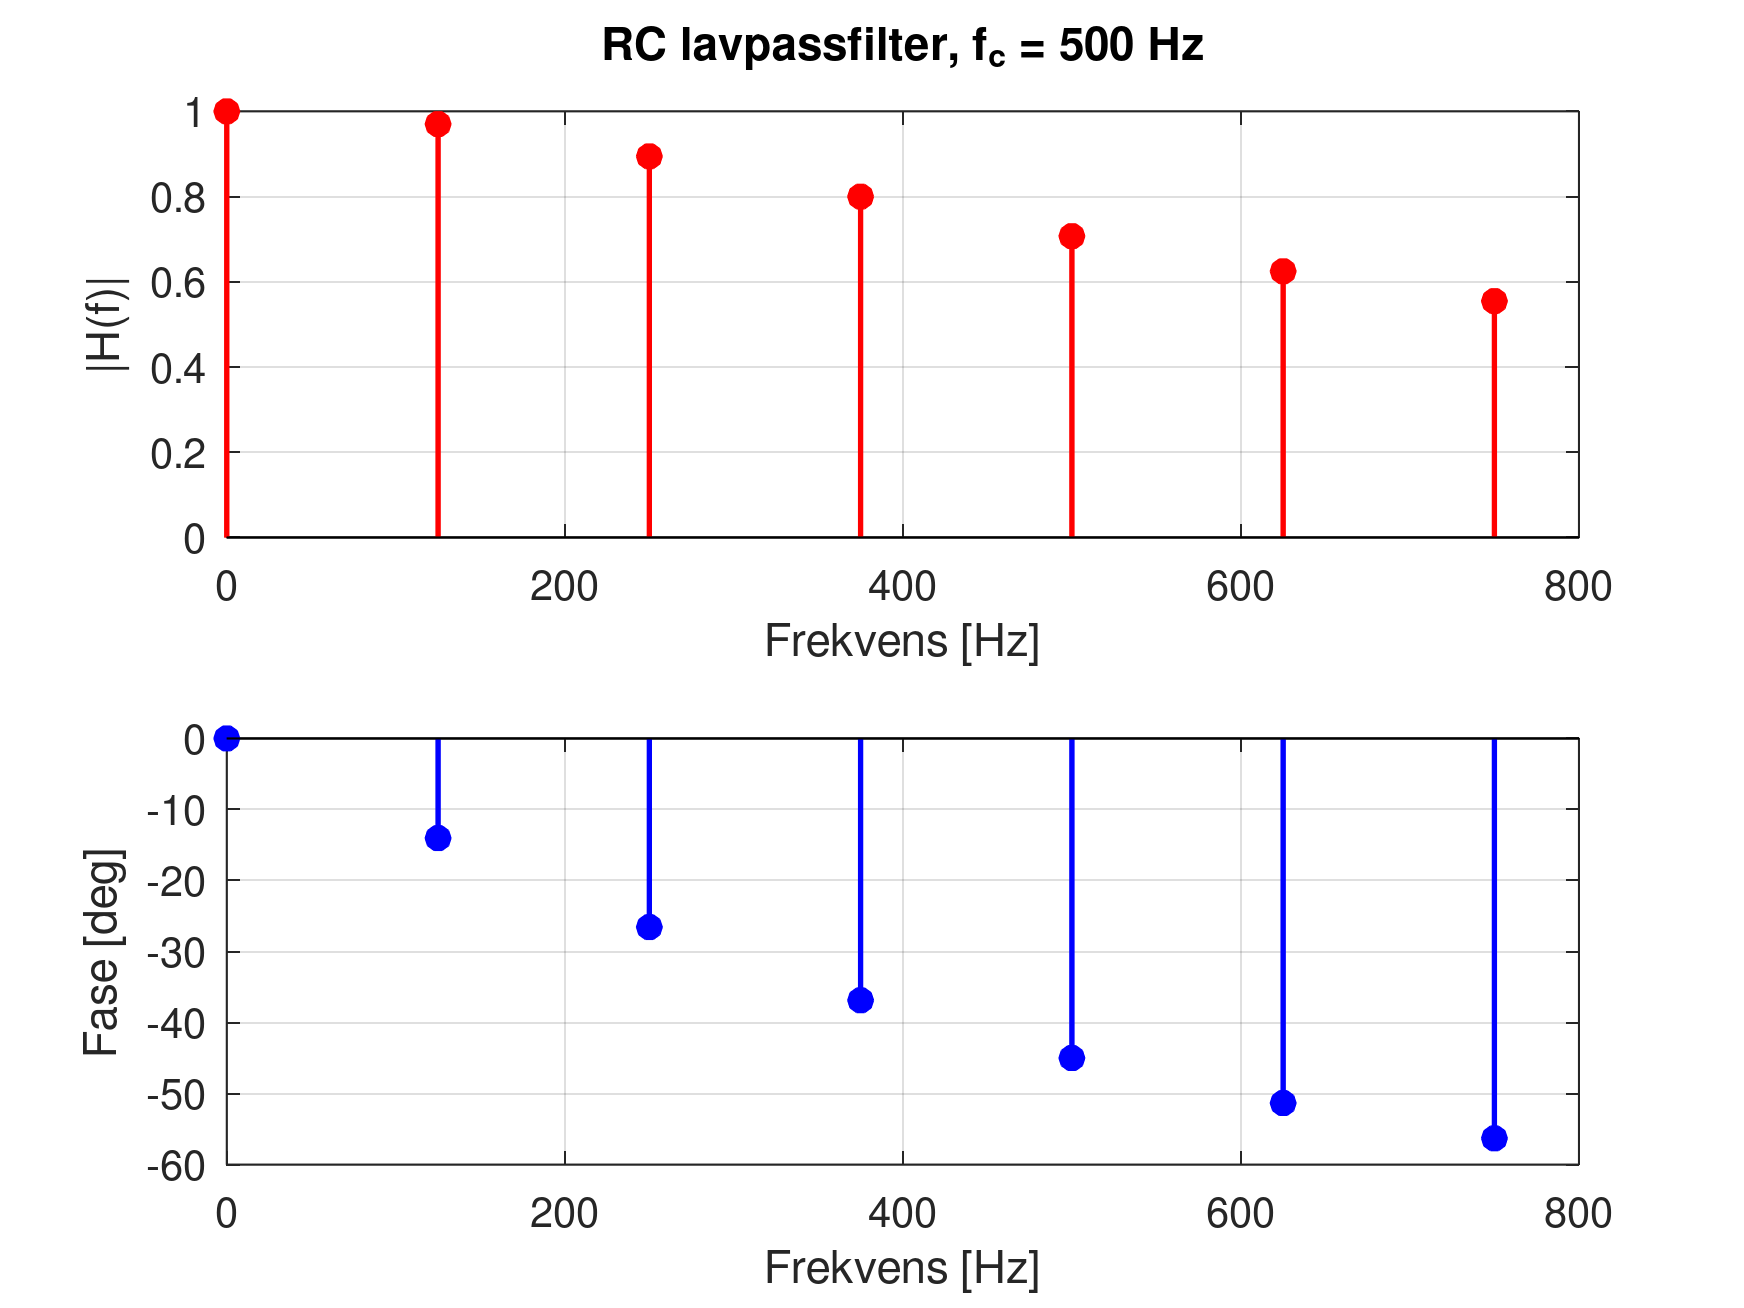
\includegraphics[width=0.85\textwidth]
    {../Media/oppgave_e_filterrespons.png}
    \caption{RC-filterets amplitude- og faserespons ved de aktuelle Fourier-frekvensene.}
\end{figure}
% --------------------------------------------------
\hypertarget{f}{}
\subsection*{f)}
Hver Fourier-komponent påvirkes forskjellig av filteret.
Amplituden til hver komponent multipliseres med filterets
amplituderespons,
\[
A_{n,\mathrm{ut}}
=
A_{n,\mathrm{inn}} \cdot 
|H(f_n)|,
\]
mens filterets faseforskyvning legges til signalets opprinnelige
fase,
\[
\phi_{n,\mathrm{ut}}
=
\phi_{n,\mathrm{inn}}
+
\angle H(f_n)
\]
\clearpage
\noindent
Dette gjøres i Octave med:
\begin{verbatim}
filtered_amp_l = gain_l .* unfiltered_amp_l;
filtered_phi_l = filter_phi_l + unfiltered_phi_l;
\end{verbatim}
Det totale utsignalet finnes deretter ved superposisjon:
\[
y(t)
=
a_0
+
\sum_{n=1}^{N}
A_{n,\mathrm{ut}} \cdot
\cos
\left(
2\pi f_nt
+
\phi_{n,\mathrm{ut}}
\right)
\]
Tabellen under viser filtrerte Fourier-koeffisienter etter filteret:
% Frekvens [Hz] | Amplitude [V] | Fase [deg] | k <= 10
%           0     0.5000          0
%    125.0000     0.8734   -14.0362
%    250.0000     0.5694   -26.5651
%    375.0000     0.2401   -36.8699
%    500.0000     0.0000   -45.0000
%    625.0000     0.1125  -231.3402
%    750.0000     0.1177  -236.3099
\begin{center}
\begin{tabular}{c|c|c|c}
$n$ & $f$ [Hz] & $A_{n, \mathrm{ut}}$ [V] & $\phi_{n, \mathrm{ut}}$ [deg] \\
\hline
0 & 0   & 0.5000  & 0 \\
1 & 125 & 0.8734  & -14.0362 \\
2 & 250 & 0.5694  & -26.5651 \\
3 & 375 & 0.2401  & -36.8699 \\
4 & 500 & 0       &  uDef \\
5 & 625 & 0.1125  & -231.3402 \\
6 & 750 & 0.1177  & -236.3099
\end{tabular}
\end{center} 
DC-komponenten påvirkes ikke av filteret siden:
\[
H(0)=1
\]
De høyere frekvenskomponentene dempes mer enn de lave
frekvenskomponentene. I tillegg får komponentene en
frekvensavhengig faseforskyvning.
\begin{figure}[H]
    \centering
    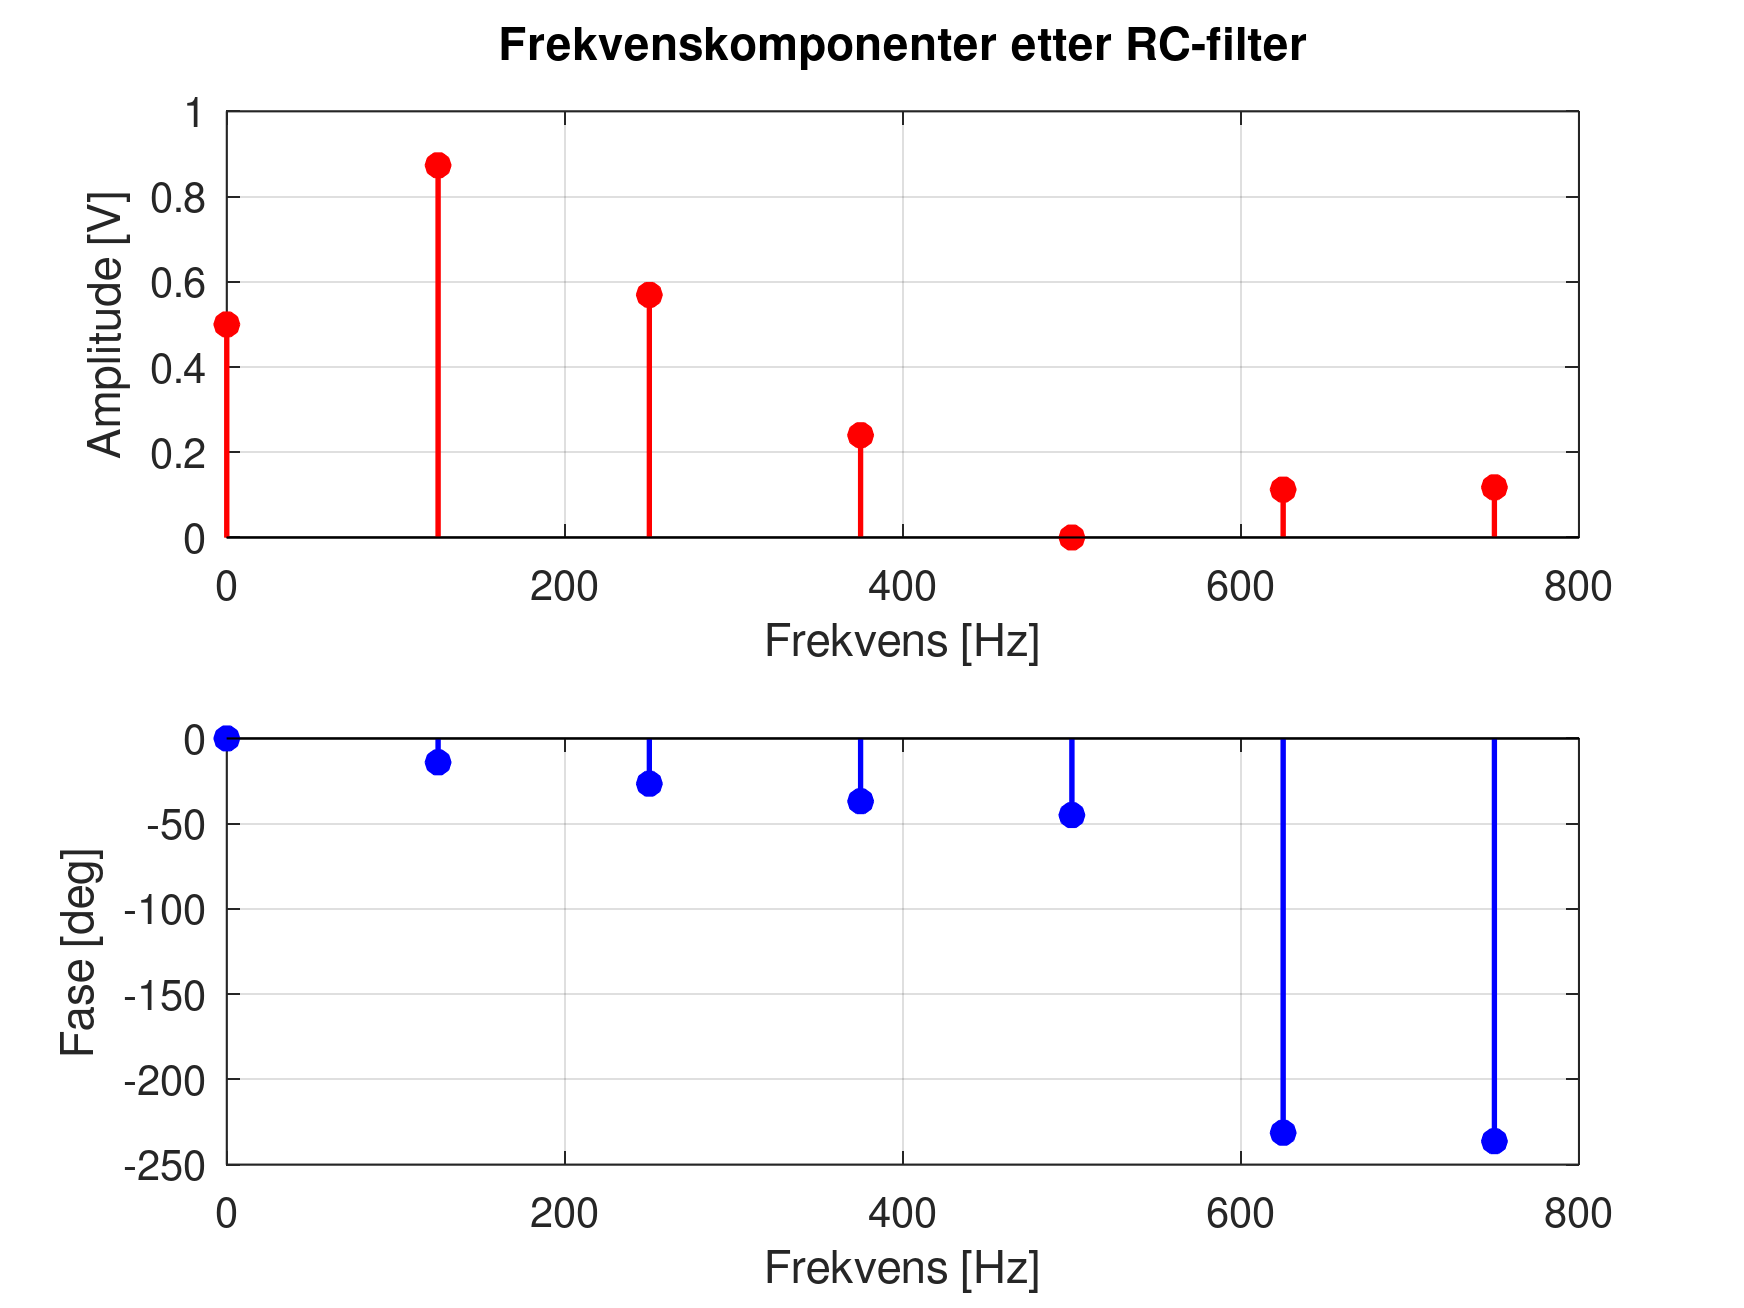
\includegraphics[width=0.75\textwidth]
    {../Media/oppgave_f_filtrert_spekter.png}
    \caption{Frekvenskomponentene etter RC-lavpassfilteret.}
\end{figure}
\noindent Det opprinnelige pulstoget, Fourier-serien før filteret og
Fourier-serien etter filteret er vist i figuren under.
\begin{figure}[H]
    \centering
    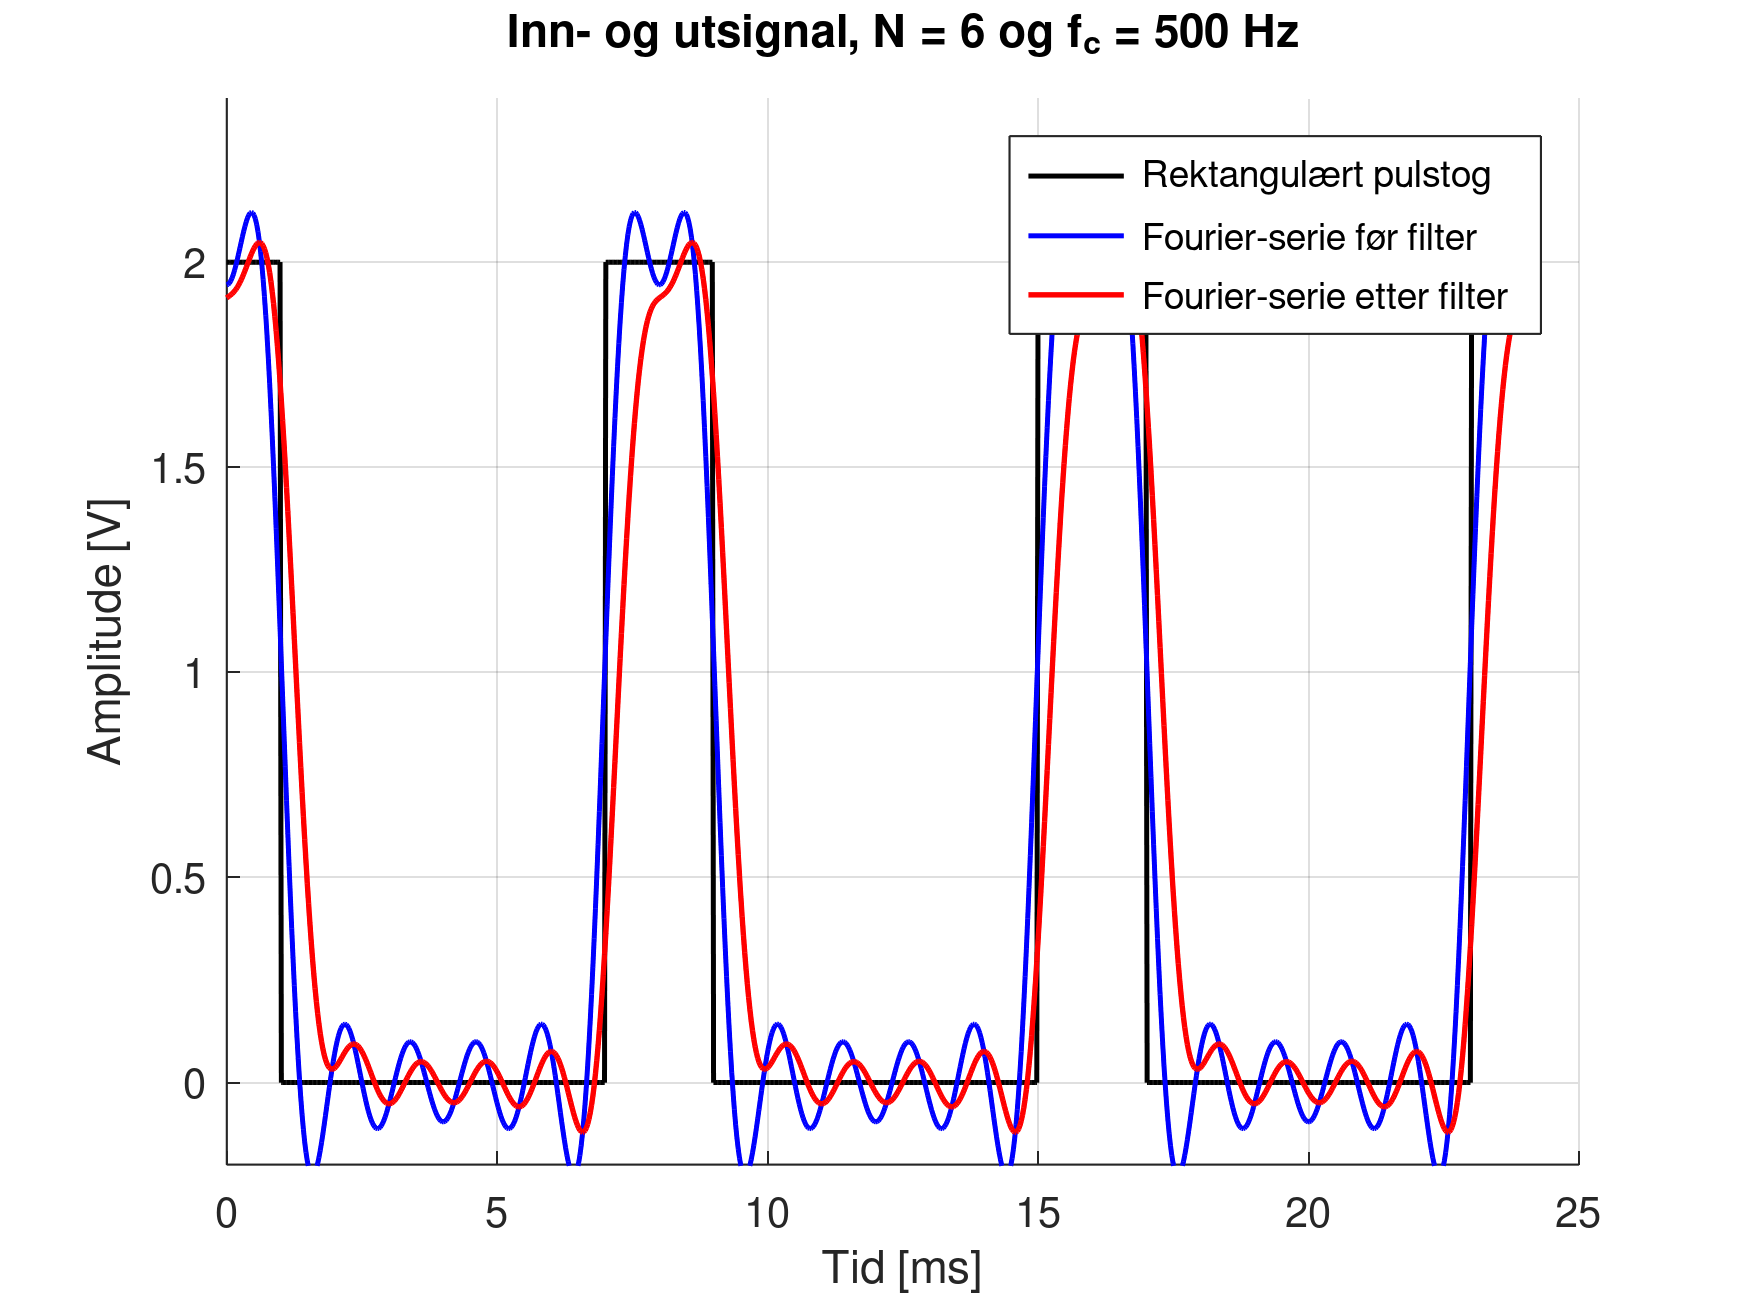
\includegraphics[width=0.9\textwidth]
    {../Media/oppgave_f_inn_og_utsignal.png}
    \caption{Sammenligning av pulstoget og Fourier-serien før og etter RC-filteret.}
\end{figure}
\noindent Det filtrerte signalet har betydelig rundere flanker enn
innsignalet. Dette skyldes at de høyfrekvente komponentene,
som er nødvendige for å lage de raske overgangene i det
rektangulære signalet, blir dempet av lavpassfilteret.
Faseforskyvningen bidrar også til at formen på utsignalet
endres.

% --------------------------------------------------
\hypertarget{g}{}
\subsection*{g)}
Både knekkfrekvensen og antall Fourier-komponenter påvirker
resultatet. En lav knekkfrekvens fører til at flere av de harmoniske
komponentene dempes kraftig. Utsignalet blir derfor glattere
og får langsommere overganger.\\[1em]
Når knekkfrekvensen økes, slipper flere av de harmoniske
komponentene gjennom filteret. Utsignalet blir da mer likt
det opprinnelige rektangulære pulstoget og får brattere
flanker.\\[1em]
Antallet Fourier-komponenter $N$ bestemmer samtidig
båndbredde til Fourier-serietilnærmingen til signalet før filtrering. Et større $N$
gir en bedre representasjon av det opprinnelige pulstoget.\\[1em]
Dersom $N$ økes mens knekkfrekvensen holdes lav, vil de nye
høyfrekvente komponentene i stor grad bli fjernet av filteret.
Forskjellen på utsignalet blir derfor mindre enn forskjellen
på innsignalet.\\[1em]
For å få et signal med svært bratte flanker må man derfor både
ha mange Fourier-komponenter og et filter med tilstrekkelig høy
knekkfrekvens.